\section{Voraussetzungen}
Um eine Aussage darüber treffen zu können, wie relevant ein Forum für ein Unternehmen ist, muss dieses Forum durchsuchbar gemacht werden.
Vorraussetzung für ein programmtechnisches Durchsuchen eines Forums ist ein erfolgreicher Login. Entweder mit einem vorhandenen Nutzeraccount oder durch eine automatische Registrierung, gefolgt von einem Login mit den gerade erstellten Daten.
Der Login in das Forum ist nötig um den geschützten Inhalt des Forums für das Programm sichtbar zu machen. Deshalb wird in diesem Kapitel die Theorie für ein erfolgreiches Registrieren und Einloggen in einem Forum beschrieben. Dazu wurden die Registrierungs- und Loginseiten von 100 Foren analysiert, die aus den Suchtreffern von Google, bei dem Suchwort `Forum`, zufällig ausgewählt wurden.

%%%%%%%%%%%%%%%%%%%%%%%%%%%%%%%%%%%%%%%%%%%%%%%%%%%%%%%%%%%%%%%%%%%%%%%%%%
%%%%%%%%%%%%% Register %%%%%%%%%%%%%%%%%%%%%%%%%%%%%%%%%%%%%%
%%%%%%%%%%%%%%%%%%%%%%%%%%%%%%%%%%%%%%%%%%%%%%%%%%%%%%%%%%%%%%%%%%%%%%%%%
\subsection {Automatisches Registrieren in Foren}
Um an den Inhalt eines Forums zu gelangen, muss in den meisten Fällen zunächst ein Nutzerprofil in dem jeweiligen Forum angelegt werden. Anschließend kann sich mit dem Profil eingeloggt und der geschützte Inhalt des Forums als Nutzer eingesehen werden. \\
Im Folgenden werden die Schritte erläutert, die ein automatisiertes Registrieren auf Webseiten ermöglichen.
Eine Übersicht zu dem Registrierungsprozess ist im Anhang (Abbildung 21) zu sehen.

\subsubsection{Ermittlung der relevanten Formulare in HTML-Webseiten}
Auf der entsprechenden Registrierungsseite des jeweiligen Forums wird eine Analyse des HTML-Quellcodes der Seite durchgeführt.
Für jedes gefundene Form-Element wird berechnet, mit welcher Wahrscheinlichkeit es die Input-Elemente für den späteren Registrierungsaufruf enthält. \\
Es werden Punkte vergeben, wenn sich in den Attributen des Form-Elements bestimmte Schlagworte wie `Signup`, `User`, `Register` etc. wiederfinden.
%%%%%%%%%%%%%%%%%%%%%%%%%%%%%%%%%%
%%%%%% STATISTIK %%%%%%%%%%%%%%%%%%%%%%%
%%%%%%%%%%%%%%%%%%%%%%%%%%%%%%%%%%
Diese Wörter wurden durch eine Analyse der Registrierungsseiten von 100 zufällig aus dem Internet gewählten Foren generiert . Dazu wurden auf jeder Seite das Registrierungsformular durchsucht und der Wert des `name`-Attributs gespeichert. Aus 100 Webseiten ergibt sich die folgende Verteilung:

\begin{table}[h!]
\centering 
\begin{tabular}{ | p{3cm} | p{3cm}|} \hline
\textbf{Attributname} & \textbf{Anzahl} \\ \hline
register & 53 \\ \hline
signup & 23 \\ \hline
usersignup & 7 \\ \hline
sign & 3 \\ \hline
u\_reg & 3 \\ \hline
reg & 2 \\ \hline
r & 1 \\ \hline
u & 1 \\ \hline
\end{tabular}
\caption{Verteilung der Attributnamen in Registrierungsformen in 100 Foren}
\end{table}



Außerdem handelt es sich bei dem Registrierungsformular mit hoher Wahrscheinlichkeit um ein POST-Formular, da es beim Absenden des Registrierungsversuches die eingegebenen Informationen wie `Nutzername`,` Passwort` und `Email` im POST-Body übermitteln muss.
Deshalb kann man sich bei den Webseiten darauf verlassen, dass, wenn Eingabefelder für das Registrieren vorhanden sind, diese sich in einem solchen POST-Formular befinden.

\begin{table}[h!]
\centering 
\begin{tabular}{ | p{5cm} | p{3cm}|} \hline
\textbf{Registrierungsform} & \textbf{Anzahl} \\ \hline
Post Formular & 89 \\ \hline
Javascriptfunktionen & 7 \\ \hline
keine Registrierung & 4 \\ \hline
\end{tabular}
\caption{Verteilung der Registrierungsformularformen in 100 Foren}
\end{table}


Ist das Registrierungsformular gefunden, werden die darin vorhandenen Input-Felder analysiert und danach gewichtet, welches Feld für Nutzernamen, Passwort und Emailadresse am wahrscheinlichsten ist.
Diese Klassifizierung erfolgt ähnlich wie bei den POST-Formularen der HTML-Webseiten anhand bestimmter Schlagworte.
So sind Input-Felder, die in ihren Attributen Wörter wie `Login`, `Username` oder `User` enthalten, wahrscheinlich die Felder, in die der Nutzername eingetragen werden soll. Demnach wird für jedes Vorkommen eines dieser Wörter der `Nutzernamen-Wahrscheinlichkeit` ein fester Wert aufaddiert. Je höher der Wert am Ende der Analyse ist, desto wahrscheinlicher handelt es sich bei diesem Input-Feld um das Feld, in das der Nutzername eingetragen werden soll. Sollten hingegen in den Attributen Wörter wie `Password` oder `Email` vorkommen, wird der `Passwort- oder Email-Wahrscheinlichkeit` des gerade betrachteten Input-Feldes ein Wert hinzuaddiert.

%%%%%%%%%%%%%%%%%%%%%%%%%%%%%%%%%
%%%%%% STATISTIK %%%%%%%%%%%%%%%%%%%%%
%%%%%%%%%%%%%%%%%%%%%%%%%%%%%%%%

\begin{table}[h!]
\centering 
\begin{tabular}{ | p{7cm} | p{3cm}|} \hline
\textbf{Name des Nutzernamenparameters} &\textbf{Anzahl} \\ \hline
username & 42 \\ \hline
name & 21 \\ \hline
login & 17 \\ \hline
userlogin & 14 \\ \hline
fullname & 2 \\ \hline
\end{tabular}
\caption{Verteilung der Nutzernamenparameter in 100 Foren}
\end{table}

Tabelle 3 zeigt, dass 4 Webseiten keine Registrierung erforderten.
10 Webseiten verlangten keine Angabe eines Nutzernamens, sondern nur die Angabe einer Email und eines Passworts. Der Name des Emailparameters ist in der Verteilung in Tabelle 3 mit enthalten.

\begin{table}[h!]
\centering 
\begin{tabular}{ | p{7cm} | p{3cm}|} \hline
\textbf{Name des Passwortparameters} & \textbf{Anzahl} \\ \hline
password & 91 \\ \hline
pass & 3 \\ \hline
pwd & 2 \\ \hline
\end{tabular}
\caption{Verteilung der Passwortparameternamen in 100 Foren}
\end{table}

\begin{table}[h!]
\centering 
\begin{tabular}{ | p{7cm} | p{3cm}|} \hline
\textbf{Name des Emailparameters} & \textbf{Anzahl} \\ \hline
email & 88 \\ \hline
mail & 5 \\ \hline
useremail & 2 \\ \hline
\end{tabular}
\caption{Verteilung der Emailparameternamen in 100 Foren}
\end{table}

5 Webseiten erforderten für die Registrierung keine Angabe einer Emailadresse.
%%%%%%%%%%%%%%%%%%%%%%%%%%%%%%%%%


Zum Schluss wird die Klassifizierung des Input-Feldes anhand der höchsten Wahrscheinlichkeit von `Email`-, `Passwort`- und \\`Nutzernamen-Wahrscheinlichkeit` vorgenommen. \\
Sind alle Input-Felder klassifiziert, werden die Checkboxen, sofern sich welche in dem Formular befinden, analysiert. Diese sind dazu da, die Foren-AGBs zu akzeptieren, angemeldet zu bleiben oder den Newsletter des jeweiligen Forums zu abonieren.
Es werden alle Checkboxen angehakt. Der Newsletter, sofern die Checkbox vorhanden sein sollte, ist nicht störend, da eine neue Spam-Email-Adresse für jedes weitere neue Registrieren in einem Forum benutzt wird.\\
Zum Schluss werden alle Inputfelder bearbeitet die `versteckt` sind, also das Attribut `hidden`, im HTML-Quellcode enthalten.
Diese Felder sind nicht dazu da, dass der Nutzer dort Informationen einträgt, sondern lediglich, um bei der Registrierungsanfrage zusätzliche Daten mitzusenden. Daher werden die Key-Value-Paare der versteckten Input-Felder zusammen mit den` Email`-, `Passwort`- und `Nutzernamendaten` der Registrierungsanfrage übergeben.

\subsubsection{Absenden der Registrierungsanfrage}
Mit dem vorherigen Schritt sind alle relevanten Daten für den Registrierungsprozess erfasst worden. Nun wird ein zufälliger Nutzername generiert. Dazu wird der externe Service randomuser.me\footnote{http://api.randomuser.me/} benutzt. Ein Aufruf dieser API liefert JSON-Informationen zu einem generierten Nutzer zurück, samt Nutzernamen. Dieser wird an die Stellen des POST-Formulars als Value des Keys eingetragen, der den Nutzernamen verlangt.\\
Im Folgenden wird ein Passwort generiert, das allen Sicherheitskriterien genügt. Das heißt Groß- und Kleinbuchstaben, Sonderzeichen und mindestens 10 Zeichen lang. Dieses wird an jede Passwort-Value-Stelle eingefügt.\\
Bei der erstmaligen Registrierung in einem Forum wird oft eine Email von dem Forum versandt, um sicherzustellen, dass der Anmelder eine valide Email bei der Registrierung angegeben hat. Das dient auch dazu, sich vor einer programmtechnischen Registrierung zu schützen. Um immer eine valide Emailadresse angeben zu können, wird ein externer Service benutzt: `10minutemail.net \footnote{https://10minutemail.net/}`, der für 10 Minuten eine valide Email-Adresse zur Verfügung stellt. Diese Email-Adresse wird als Value in Email-Input-Felder eingetragen.\\
Nun sind alle Key-Value Paare im POST-Body der Registrierungsanfrage valide und die Anfrage kann abgesendet werden.
Die URL, an die der Registrierungsversuch gesendet wird, setzt sich aus der Top-Level-Domain der Webseite und der `action`-Value des POST- Formulares, sowie dem generierten POST-Body, zusammen.

\subsubsection{Bestätigen des Registrierungslinks in der Registrierungs-Email}
Nachdem die Registrierungsaufforderung im Forum eingeht, wird eine Bestätigungsmail an die Email-Adresse gesendet.
Um diese Email nun abrufen zu können, wird alle 5 Sekunden die `10minute.net`-Email-Webseite neu geladen, damit eine etwaige neue Email angezeigt wird. Da die Seite keinen Login erfordert, wird die Zuordnung zwischen Nutzer und zugehörigen Emails über Cookies gelöst. Diese Cookies werden beim ersten Besuch der Webseite im Response-Header an den Nutzer mit übergeben. Wenn bei dem programmtechnischen Neuladen der Webseite diese Cookies mitgesendet werden, können Emails, die an die Adresse gesendet wurden, abgerufen werden. Bei einem Fehlen der Cookies würde immer eine neue Emailadresse angelegt werden.\\
Wird nun die Email des Forums in dem Posteingang gefunden, werden alle Hyperlinks aus dem Email-Inhalt extrahiert und einmal mit einem `GET-Request` aufgerufen. Das sichert, dass das angelegte Nutzerprofil in dem Forum aktiviert, validiert und zum Einloggen freigeschaltet wird.

%%%%%%%%%%%%%%%%%%%%%%%%%%%%%%%%%%%%%%%%%%%%%%%%%%%%%%%%%%%%%%%%%%%%%%%%
%%%%%%%%%%%%% LOGIN %%%%%%%%%%%%%%%%%%%%%%%%%%%%%%%%%%%%%
%%%%%%%%%%%%%%%%%%%%%%%%%%%%%%%%%%%%%%%%%%%%%%%%%%%%%%%%%%%%%%%%%%%%%%%%

\subsection {Automatisches Einloggen in Foren}
Der Login ist wichtig, um die Cookies der Webseite zu erhalten, die dann bei jeder neuen Anfrage an die Webseite wieder mitgesendet werden müssen, um zu validieren, dass die Anfrage von einem eingeloggten Nutzer stammt. Damit wird der geschützte Bereich des Forums zugänglich.
Eine Übersicht zu dem Loginprozess kann im Anhang (Abbildung 22) gefunden werden.

\subsubsection{Ermittlung der relevanten Formulare in HTML-Webseiten}
Die Ermittlung der relevanten Login-Form sowie von Input-Feldern erfolgt nach dem Prinzip der Suche nach den relevanten Registrierungsformularen. Es werden zuerst alle POST-Formulare des HTML-Quellcodes extrahiert und bewertet. Der Unterschied besteht darin, dass die Anzahl der Input-Felder in der Form zwischen 2 und 3 liegen müsste, da als Maximum Email, Nutzername und Passwort angegeben werden müssen. Das Minimum ist hingegen Nutzername oder Email und das Passwort. Alle Formulare mit mehr Eingabemöglichkeiten sind höchst wahrscheinlich nicht das Login-Formular.
Sollte es mehr als ein Formular geben, das zwischen 2 und 3 Input-Feldern besitzt, müssen die Input-Felder genauer betrachtet werden. \\
Enthalten diese in ihren Attributen differenzierte Schlagworte wie `login`, `username`, `passwort` oder `email`, werden für jedes Auftreten dieser Schlagworte Punkte auf den Punktewert dieser Form aufgerechnet.


Weiterhin werden die Input-Typen der Input-Formen analysiert. Bestehen sie aus den Kombinationen Input-Typ = 'text' und Input-Name = Einer Kombination aus den Worten `login`, `username` oder `email`, werden weitere Punkte zu dem Punkewert hinzugerechnet (Tabelle 6).
\[Inputtype = `text` \wedge Inputname \subseteq \{`login`,`username`,`email`\}\]

\begin{table}[h!]
\centering 
\begin{tabular}{ | p{3cm} | p{3cm}|} \hline
\textbf{Attributname} & \textbf{Anzahl} \\ \hline
login & 79 \\ \hline
email & 20 \\ \hline
username & 16 \\ \hline
password & 3 \\ \hline
andere & 5 \\ \hline
\end{tabular}
\caption{Verteilung der Attributnamen in Loginformen in 100 Foren, mit Input-Typ = `text`}
\end{table}



Gleiches gilt für eine Kombination aus Input-Typ = `password` und Input-Namen = `password` (Tabelle 7).
\[Inputtype = `password` \wedge Inputname = `password`\]

\begin{table}[h!]
\centering 
\begin{tabular}{ | p{3cm} | p{3cm}|} \hline
\textbf{Attributname} & \textbf{Anzahl} \\ \hline
password & 83 \\ \hline
pass & 3 \\ \hline
pwd & 2 \\ \hline
andere & 5 \\ \hline
\end{tabular}
\caption{Verteilung der Attributnamen in Loginformen in 100 Foren mit Input-Typ `password`}
\end{table}

4 der Foren, bei denen keine Registrierung notwendig war, benötigen auch keinen Login. Bei den fehlenden 3 Foren hatte das Passwort den Input-Typ `text`.
Sollte die Form genau ein Input-Feld mit dem Typ `password`, ein Input-Feld mit dem Typ `text ` und eine Checkbox haben, ist diese Form am wahrscheinlichsten die Login-Form. Sie bestünde aus einem Feld für den Usernamen oder Email, einem Passwortfeld und einer Checkbox, ob ein Angemeldet-Bleiben erwünscht ist. Aus den 100 getesteten Webseiten bestanden 66\% der Loginseiten aus diesem Schema.

Sind alle Formen auf der Seite analysiert, wird die Form mit der höchsten Wahrscheinlichkeit für den Login-Request benutzt. Eine Klassifizierung der Input-Felder, ob sie den Usernamen, Email oder Passwort übermitteln, wurde im vorherigen Schritt schon angelegt, da sich daraus der Form-Score berechnet. Zum Schluss werden noch alle zusätzlichen Input-Felder, die die Eigenschaft `visibility = hidden` haben, als Key-Value-Paar zusammen mit den Namen der Email-, Passwort- und Nutzername-Felder und deren Klassifizierung im JSON-Format gespeichert.

\subsubsection{Absenden des Loginrequests}
Der Request, der an das Forum abgesendet wird, ist ein POST-Request, da er die Formulardaten an das Forum mit übermitteln muss.
An die Value-Stelle der klassifizierten Input-Namen werden Daten wie Password, Email und Nutzername eingetragen und das Forum gesendet.
Sollte dieser Request scheitern, werden die restlichen Formen, die sich aus dem HTML-Quellcode extrahieren ließen, als mögliche Login-Formen ausprobiert.

\subsubsection{Handhabung von Cookies und Redirects}
Sollte in dem Response-Header des Forums bei einer Loginanfrage ein Statuscode 200 gesendet werden, war der Loginversuch erfolgreich. Da das HTTP-Protokoll keine Zustände speichern kann, muss dem Forum bei jeder neuen Anfrage mitgeteilt werden, dass die Anfrage nach einem erfolgreichen Loginversuch unternommen wurde. Andernfalls würde das Forum den Zugriff auf die Daten, die nach einem erfolgreichen Login eingesehen werden können, sperren.\\
Um das zu gewährleisten, werden die Cookies aus dem Response-Header der erfolgreichen Loginanfrage gespeichert und bei jeder neuen Anfrage an das Forum mitgesendet.\\
Sollte in dem Response-Header ein Feld `Location` existieren, bedeutet das, dass es einen Redirect nach dem Login gibt, bei dem der Browser eine andere URL lädt. Dieser Redirect ist für den nachfolgenden Schritt, das Suchen des Suchformulares in Foren, wichtig. Das Suchformular befindet sich bei 100 getesteten Foren bei 93\% der Foren auf der Hauptseite. Ein Redirect führt in den meisten Fällen zu genau dieser Hauptseite des Forums. Deshalb wird die URL, die sich in dem Location-Header befindet, durch einen `GET-Request` geladen und für die weitere Verarbeitung genutzt. Das stellt sicher, dass sich ein Such-Formular in dem zu analysierenden HTML-Quellcode befindet.

%%%%%%%%%%%%%%%%%%%%%%%%%%%%%%%%%%%%%%%%%%%%%%%%%%%%%%%%%%%%%%%%%%%%%%%%
%%%%%%%%%%%%% SUCHEN %%%%%%%%%%%%%%%%%%%%%%%%%%%%%%%%%%%%%
%%%%%%%%%%%%%%%%%%%%%%%%%%%%%%%%%%%%%%%%%%%%%%%%%%%%%%%%%%%%%%%%%%%%%%%%
\section{Forenrelevanz}
\subsection{Ermitteln der Größe der Forendatenbank}
Die Ermittelung der Datenbankgröße wird bei dem späteren Treffen der Aussage über die Forenrelevanz für ein Produkt relevant.
Es ist wichtig, die ungefähre Anzahl der Beiträge in dem Forum zu kennen, um eine Aussage darüber zu treffen, wie das Verhältnis zwischen Datenbankgröße und produktspezifischem Beitrag ist. Ist dieses Verhältnis zu klein, lohnt es sich nicht, dieses Forum zu durchsuchen, da die Zeit, einen Produktpost zu finden, der noch dazu einen Kaufwillen ausdrückt, zu lang ist und sich das Suchen nicht rentieren würde.
Eine Übersicht zu dem Suchprozess kann am Ende des Kapitels in Abbildung 1 gefunden werden.	

\subsubsection{Ermitteln des Suchfeldes}
Um die Datenbank analysieren zu können, muss zunächst das Suchfeld gefunden werden, das es in den meisten Foren gibt, um die vorhandenen Beiträge zu durchsuchen.
Dazu wird das HTML nach dem erfolgreichen Einloggen auf weitere Form-Felder durchsucht. Die gefundenen Felder werden klassifiziert, indem sich die Namen-Attribute der Input-Felder dieser Form angeschaut werden. Sollte dieser Name aus einem `q` oder `search` bestehen (Tabelle 8), werden Punkte vergeben. Das `q` steht bei den meisten Webseiten für den Paramater `query`, der das Suchwort überträgt.
Danach werden alle Attribute der Input-Felder der Form durchsucht. Sollten in den Attributen die Zeichenketten `search` oder `suche` vorkommen, werden weitere Punkte vergeben.

\begin{table}[h!]
\centering 
\begin{tabular}{ | p{3cm} | p{3cm}|} \hline
\textbf{Attributname} & \textbf{Anzahl} \\ \hline
q & 53 \\ \hline
search & 24 \\ \hline
suche & 5 \\ \hline
andere & 18 \\ \hline
\end{tabular}
\caption{Verteilung der Attributnamen in Suchformen in 100 Foren}
\end{table}

Zum Schluss ist die Form mit dem höchsten Punktwert die Form, die am wahrscheinlichsten die Suchbar als Input-Feld enthält.
Nun wird der Pfad der Suchanfrage aus der Form extrahiert, indem das `action`-Attribut der Form ausgelesen wird. Dieser Wert wird an die Toplevel-Domain angefügt und stellt die Such-URL dar. Der Queryparameter wird aus dem Namen-Attribut des Input-Feldes extrahiert und an die Such-URL angehängt. Sollte zum Beispiel das Namen-Attribut des Input-Feldes ein `q` sein, würde sich die vorläufige Such-URL folgendermaßen zusammensetzen:

\[ URL := `Domainname` + action + ?q= \]

An den Queryparameter `q` werden im Folgenden die einzelnen Suchworte, die zur Ermittelung der Datenbankgröße beitragen, angehängt und an das Forum gesendet.\\
Die Wörter, die die Datenbank bestimmen sollen, werden aus einer Datei gelesen, die die am häufigsten benutzten Wörter einer Sprache sortiert auflistet. Daraus werden zufällig 500 Wörter gezogen ,in die URL eingefügt und abgesendet.

\subsubsection{Berechnung der Datenbankgröße}
Nach jeder abgesendeten Anfrage wird der zurückgegebene Inhalt analysiert. Dieser enthält die Beiträge, die von der 
forumseigenen Suchmaschine zurückgegeben werden, wenn man nach einem spezifischen Wort sucht. Im betreffenden Inhalt werden alle Hyperlinks gesucht und gespeichert. Diese Prozedur wird 500 mal wiederholt. Zum Schluss wird die Gesamtzahl an gewonnenen Links berechnet sowie die Anzahl der Links, die bei unterschiedlichen Suchwörtern identisch sind. Links, die in mehr als 50\% der Gesamtanfragen vorkommen, werden ignoriert, da es sich hierbei meist um statische Links handelt, die sich auf der Suchseite befinden. Diese Links zeigen nicht auf Beiträge, die aus der Suchanfrage generiert werden, sondern auf statische Elemente der HTML-Webseite wie Navigationsbar oder Ähnliches. Sie würden dann die Berechnung der Datenbankgröße verfälschen und werden deshalb ignoriert.
Die finale Größe der Datenbank lässt sich mit Hilfe der Formel \[|DB_{Gesamt}| = \frac{u}{1-OR^{-1.1}}\] berechnen. Hierbei bedeutet \textit{u} die Anzahl der einmaligen Dokumente und \textit{OR} das Verhältnis von allen zu doppelten Dokumenten. Das Verhältnis von einmaligen zu doppelten Dokumenten bestimmt die Datenbankgröße\cite{lu2008efficient}.\\
Dieser Vorgang wird drei Mal wiederholt und aus den drei resultierenden Datenbankgrößen wird das arithmetische Mittel gebildet. Diese Zahl bestimmt, wie viele Beiträge sich insgesamt in der Forendatenbank befinden.

%%%%%%%%%%%%%%%%%%%%%%%%%%%%%%%%%%%%%%%%%%%%%%%%%%%%%%%%%%%%%%%%%%%%%%%%
%%%%%%%%%%%%% FORENRELEVANZ %%%%%%%%%%%%%%%%%%%%%%%%%%%%%%%%%%
%%%%%%%%%%%%%%%%%%%%%%%%%%%%%%%%%%%%%%%%%%%%%%%%%%%%%%%%%%%%%%%%%%%%%%%%


\subsection{Ermitteln der Forenrelevanz}
Um eine gezielte Aussage darüber treffen zu können, ob das gerade analysierte Forum überhaupt relevant für die Verkaufsstrategie eines Unternehmens ist, müssen neben der Gesamtgröße des Forums auch Anzahl und Qualität der Beiträge für Verkaufsprodukte analysiert werden. Das Verhältnis von Gesamtforengröße, Beitragsanzahl zu jedem einzelnen Unternehmensprodukt und die Qualität der Beiträge, gemessen an dem ausgedrückten Bedürfnis, etwas zu kaufen, gibt Aufschluss darüber, ob das Forum für eine Firma als wichtig erachtet werden kann.


\subsubsection{Generierung der Produktschlagworte}
Die Ermittelung der Gesamtanzahl der Beiträge, die einem Firmenprodukt zugeordnet werden, erfolgt in der gleichen Art und Weise wie die Ermittlung Gesamtgröße der Forendatenbank.\\
Zu diesem Zweck werden Dokumente der Firmen analysiert, die eindeutig ein Produkt beschreiben. Das können Broschüren, Webseiten oder PDF-Dateien sein, die von der jeweiligen Firma hochgeladen wurden. Aus diesen Texten werden die häufigsten Wörter nach Tf-idf-Maß extrahiert. In der generierten Wortliste werden z.B Füllwörter oder andere `allgemeine` Begriffe entfernt\footnote{http://xpo6.com/list-of-english-stop-words/ besucht: 25.06.2015}, die, wenn sie gesucht werden,  beliebige Beiträge als Suchergebnis liefern würden, deren Inhalt nichts mit dem eigentlich gesuchten Produkt zu tun hat.\\
Ist die Wortliste generiert, werden diese Worte mit Hilfe der Suchmaske des Forums gesucht und die Links in der Antwort gespeichert und gezählt. Hinzu kommt, dass jeder gefundene Link zu einem Beitrag durch einen weiteren `GET-Request` an diese Seite aufgerufen und heruntergeladen wird. Die heruntergeladene Seite gibt den selben Zustand wieder, als wenn sich ein Mensch mit dem Browser einloggt und diesen Beitrag aufrufen würde. Aus dem Dokument werden alle HTML-Tags entfernt. Der Inhalt ist der erste zusammenhängende Text, der 40 oder mehr Zeichen enthält \footnote{http://blog.viermalvier.at/die-richtige-laenge-von-social-media-postings-mit-infografik/ besucht: 25.06.2015}, da das die optimale Anzahl an Buchstaben in einem Social-Media-Beitrag darstellt.

\subsubsection{Analyse der Forenbeiträge}
Ist der Inhalt extrahiert, wird er durch einen Klassifizierungsservice auf Grund der zuvor hochgeladenen Firmenbroschüren bewertet. Die Broschüren beschreiben genau ein Produkt im Detail. Die Gesamtheit aller Broschüren, die ein Produkt klassifizieren, bilden Produktcluster. Jeder Eintrag verweist mit einem Distanzvektor auf die ihm nächsten ähnlichen Broschüreneinträge. Soll nun ein gerade gewonnener Beitragsinhalt klassifiziert werden, werden die ihm ähnlichsten Broschüreneinträge berechnet. Über den `K-Nearest-Neighbour-Algorithmus` wird nun bestimmt, welchem Produkt der Text des Beitrags am ähnlichsten ist. Ist der Beitrag einem bestimmten Produkt zugeordnet, wird anschließend der in dem Beitrag zum Ausdruck gebrachte Kaufbedarf berechnet. Dieses geschieht mit einer Support-Vektor-Maschine, die von Hennig und Berger entwickelt wurde \cite{n2o}.\\
Wird ein Beitrag einem Produkt zugeordnet und drückt dieser Beitrag einen Kaufwillen aus, wird er für die weitere Berechnung der Relevanz des Forums in Betracht gezogen.

\subsubsection{Ermittelung der Datenbankgröße je Unternehmensprodukt}
Die Links der Beiträge, die sowohl ein Produkt als auch einen Kaufwillen ausdrücken, werden gespeichert. Die Ermittlung der Datenbankgröße je Unternehmensprodukt erfolgt analog zu der Ermittlung der Gesamtdatenbankgröße des Forums. Die Formel \[|DB_{Produkt}| = \frac{u}{1-OR^{-1.1}}\] \cite{lu2008efficient} liefert auch hier die Größe der Datenbankeinträge, abgeschätzt aus dem Verhältnis von einmaligen zu sich überschneidenden Beiträge, zurück.
Sollten mehr als 30\% der analysierten Beitragsinhalte zu einem Unternehmensprodukt einen Verkaufsbedarf ausdrücken, kann dieses Forum für das Unternehmen als wichtig erachtet werden.

\newpage


\begin{figure}[h!]
\centering
		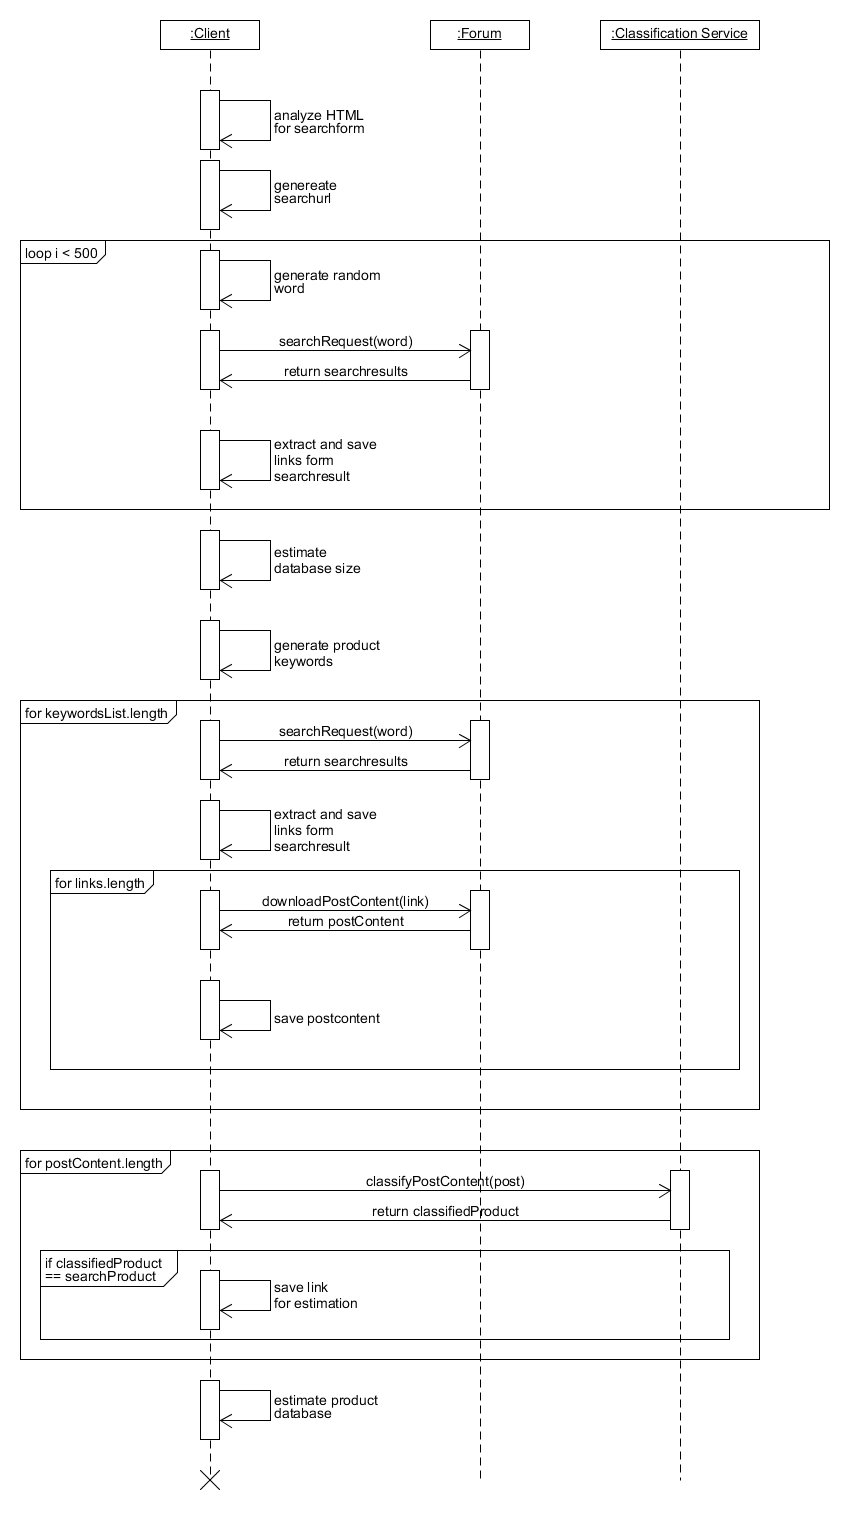
\includegraphics[width=0.75\textwidth,height=\textheight,keepaspectratio]{./diagrams/estimate_seq.png}
		\caption{Vollständiger Datenbankabschätzungsablauf}
	\end{figure}
	
	
\newpage

